
\documentclass[style=sailor,size=12pt]{powerdot}
\usepackage{epic,array,ecltree,url,calrsfs}
\usepackage[nointegrals]{wasysym}
\usepackage{listings}
\usepackage{epsfig}
\usepackage{amsmath}
\usepackage{amsfonts}
\usepackage{amssymb}
\usepackage{amsxtra}
\usepackage{amsthm}
\usepackage{mlextra} % Must be below ams packages
\usepackage{mathrsfs}
\usepackage{color}
\usepackage{array}
\usepackage{graphicx}
\graphicspath{ {../art/} }
\usepackage{bm}
\usepackage{tikz}
\usepackage{multicol}
\usepackage{enumitem}
\usepackage{blkarray}
\usepackage{bigstrut}
\setlength{\bigstrutjot}{4pt}
\usetikzlibrary{arrows}
\usepackage{subcaption}

\pdsetup{method=normal,
list={labelsep=1em,leftmargin=1cm,itemsep=0pt,topsep=5pt,parsep=0pt}
}
% import from truth and PTL.
\title{Discrete Math Review}
\author{Foundations of Computer Science}
\date{\today}

\begin{document}
\maketitle

\begin{slide}[toc=,bm=]{Overview}
This slide set covers the following topics:

\vspace{5mm}
\tableofcontents[content=sections]
\end{slide}

\section[slide=true]{Sets, Sequences, Strings} 
\section[slide=true,tocsection=false]{Sets}

\begin{slide}[bm=,toc=]{Finite and infinite Sets}

\emph{\textbf{Definition: A set is a collection of elements.}}
\pause
\begin{itemize}
   \item<2-> $a \in S$ means $a$ is an element of set $S$ 
   \item<3-> $a \notin S$ means $a$ is not an element of set $S$
   \item<4-> The \emph{cardinality} of a set $S$ is denoted $|S|$. 
   \begin{itemize}
       \item<5-> Cardinality indicates the number of elements in the set.
   \end{itemize}
   \item<6-> $\emptyset$ represents the set with no elements (``empty set'').
   \begin{itemize}
       \item<7-> $\emptyset$ has cardinality 0. 
   \end{itemize}
\end{itemize} 
\end{slide}

\begin{slide}[bm=,toc=]{Specifying Sets}
\textbf{Three ways of defining a set:}
\begin{itemize}
   \item<2-> Explict (write out the elements).
   \begin{itemize}
      \item<3-> $S = \{red, yellow, green\}$ 
      \item<4-> $R = \{1,2,3\}$
      \item<5-> This does not work for infinite sets.
   \end{itemize} 
   \item<6-> Through \emph{set comprehension}. 
   \begin{itemize}
      \item<7-> $\N = \{n| n \in \Z, n \geq 0\}$ 
      \item<8-> $E = \{n| n \in \N, n \mod{2} = 0 \}$
   \end{itemize}
   \item<9-> Through operations on sets that have already be defined. 
   \begin{itemize}
      \item<10-> $K = S \cup R = \{red, yellow, green, 1, 2, 3\}$ 
      \item<11-> See ``Operations on Sets and Strings'' for examples. 
   \end{itemize}
\end{itemize} 

\end{slide}


\begin{slide}[bm=,toc=]{Applications of sets}
Sets are the basis for:
\begin{itemize}
   \item<2-> Relations
   \item<3-> Functions
   \item<4-> Equivalence classes
   \item<5-> Partial orders
\end{itemize}
\pause[5]Important infinite sets: 
\begin{itemize}
   \item<7-> $\N$: Natural Numbers
   \item<8-> $\Z$: Integers
   \item<9-> $\Q$: Rational Numbers
   \item<10-> $\R$: Real Numbers
   \item<11-> $\C$: Complex Numbers
\end{itemize}
\end{slide}

\section[slide=true,tocsection=false]{Sequences}

\begin{slide}[bm=,toc=]{Finite and Infinite Sequences}
\pause
\begin{defn}{A.12}[Ben Ari]~\\\pause
Let $\mathcal{S}$ be a set.
\begin{itemize}
    \item<4-> A \emph{finite sequence} $f$ is a function from $\{0,...,n-1\}$ to $\mathcal{S}$.
    \begin{itemize}
        \item<5-> The length of the sequence is $n$.
    \end{itemize}
    \item<6-> An \emph{infinite sequence} $f$ on $\mathcal{S}$ is a function from $\N$ to $\mathcal{S}$.
    \end{itemize}
\end{defn}
\pause[4]
\begin{defn}{A.14}[Ben Ari]~\\\pause
Let $f$ be a sequence on $\mathcal{S}$. The sequence is denoted:
\pause
\[
  (s_0,s_1,s_2,...)
  \]
\pause
where $s_i = f(i)$.
\end{defn}
~\\
\pause
\begin{defn}{A.15}[Ben Ari]
~\\
\pause
A finite sequence of length $n$ is an \emph{n-tuple}.
\end{defn}

\end{slide}


\section[slide=true,tocsection=false]{Strings}
\begin{slide}[bm=,toc=]{Strings: Definitions}
\pause
\begin{defn}{--- Alphabet}~\\
\pause Any finite set. 
\end{defn}
\vspace{-5mm}
\begin{itemize}
\item<4-> For example $\{0,1,2,...,9\}$ and $\{0,1\}$ are alphabets. 
\item<5-> The set $\{a,b\}$ is an alphabet. 
\item<6->  $\Sigma$ denotes an arbitrary alphabet. 
\item<7->  We call the elements of $\Sigma$ \emph{letters} or \emph{symbols}.
\end{itemize}
\pause[5]
\begin{defn}{--- String}~\\
\pause
A \emph{string} over $\Sigma$ is any finite-length sequence of elements of
$\Sigma$. 
\end{defn}
\vspace{-5mm}

\begin{itemize}
\item<10-> For example, if $\Sigma = \{a,b\}$ then $aabab$ is a string of length $5$ over $\Sigma$.
\item<11-> The length of a string $x$ is denoted $|x|$. 
\item<12-> There is a unique string of length zero over any alphabet $\Sigma$ called
      the \emph{empty string} and it is denoted $\epsilon$.
\end{itemize}
\end{slide}

\begin{slide}[bm=,toc=]{$\emptyset \neq \{\epsilon\} \neq \epsilon$}
    Note that $\emptyset$, $\{\epsilon\}$ and $\epsilon$ are three different things.
    \begin{itemize}
    \item<2-> $\emptyset$ is a set with no elements.
    \item<3-> $\{\epsilon\}$ is a set with one element, namely the empty string.
    \item<4-> $\epsilon$ is a string, not a set.
    \end{itemize}
\end{slide}



\section[slide=true]{Operations on Sets and Strings}
\begin{slide}[bm=,toc=]{Set Inclusion}
\begin{defn}{A.3}[Ben Ari]
Let $S$ and $T$ be sets.
\begin{itemize}
\item $S$ is a \emph{subset} of $T$ if and only if every element of $S$ is an
      element of $T$.
\item Equivalently, $S \subseteq T$ if and only if $x \in S$ implies $x \in T$.
\item $S$ is a \emph{proper subset} of $T$, (i.e.\ $S \subset T$) if and only
      if $S \subseteq T$ and $S \neq T$.
\end{itemize}
\end{defn}
\begin{thm}{A.5}[Ben Ari]
$\emptyset \subseteq T$
\end{thm}
\begin{thm}{A.6}[Ben Ari]
\emph{The subset property is transitive.}
\end{thm}
\begin{thm}{A.7}[Ben Ari]
$S = T$ if and only if $S \subseteq T$ and $T \subseteq S$.
\end{thm}



\end{slide}

\begin{slide}[bm=,toc=]{Basic operations on sets}
\begin{itemize}
   \item \emph{Set union}: 
   \[
     A \cup B = \{x|x \in A \text{ or } x \in B\}
   \]

   \item \emph{Set intersection}: 
   \[
     A \cap B = \{x|x \in A \text{ and } x \in B\}
   \]

   \item \emph{Set difference}: 
   \[
     A - B = \{x|x \in A \text{ and } x \notin B\}
   \]

\end{itemize}
\end{slide}

\begin{wideslide}[bm=,toc=]{Illustration of Set Operations}
\vspace*{15mm}

\unitlength=1.0pt
\begin{center}
\begin{picture}(260,110)
\put(80,40){\oval(160,80)}
\put(180,40){\oval(160,80)}
\put(  0,0){\makebox(100,80){$S-T$}}
\put(100,0){\makebox( 60,80){$S\cap T$}}
\put(160,0){\makebox(100,80){$T-S$}}
\put(0,60){\makebox(20,20)[r]{S}}
\put(240,60){\makebox(20,20)[l]{T}}
\put(20,85){\makebox(220,10){$\overbrace{\hspace*{220pt}}$}}
\put(100,100){\makebox( 60,10){$S\cup T$}}
\end{picture}
\end{center}
\end{wideslide}


\begin{slide}[bm=,toc=]{Cartesian Products}
\begin{defn}{A.17}[Ben Ari]
~\\
\emph{Cartesian Product of 2 Sets:}
\begin{itemize}
\item Let $S$ and $T$ be sets.
\item We define their \emph{Cartesian Product}, $S \times T$, as the set of all
pairs $(s,t)$ such that $s \in S$ and $t \in T$.
\end{itemize}
\emph{n-ary Cartesian Product:}
\begin{itemize}
\item This is the general case.
\item Let $S_1,...,S_n$ be sets.
\item We define their \emph{Cartesian Product}, $S_1 \times \cdots \times S_n$, as the set of all
$\emph{n-tuples}$ $(s_1,...,s_n)$ such that $s_i \in S_i$.
\item If all sets $S_i$ are the same set, the notation $S^n$ is used for $S
\times \cdots \times S$.
\end{itemize}
\end{defn}
\end{slide}

\begin{slide}[bm=,toc=]{String Concatenation}

\begin{itemize}
    \item If $x$ and $y$ are strings then string $xy$ is called the
    \emph{concatenation} of $x$ and $y$.
    \item Concatenation is associative: $(xy)z = x(yz)$. 
    \item Concatenation is not commutative. $xy$ and $yx$ are different strings
    in general.
    \item $\epsilon$ is an identity for concatenation: ${\epsilon}x = x\epsilon = x$. 
    \item $|xy| = |x| + |y|$. 
    \item We write $a^n$ for a string of $a$'s of length $n$.
    \begin{itemize}
        \item For example, $a^5 = aaaaa$ and $a^0 = \epsilon$. 
        \item And $a^ma^n = a^{m+n}$ for all $m,n \geq 0.$
    \end{itemize} 
\end{itemize} 
\end{slide}

\begin{slide}[bm=,toc=]{Set Concatenation}
\emph{\textbf{Definition:}}
\begin{itemize}
   \item  $\mli{AB} = \{xy | x \in A \text{ and } y \in B\}$. 
   \item When forming a set concatenation, you form \emph{all} strings that can be obtained in this way.
   \item Example:
   \[\{\textcolor{red}{a},\textcolor{brown}{ab}\}\{\textcolor{green}{b},\textcolor{blue}{ba}\} = \
                      \{\textcolor{red}{a}\textcolor{green}{b}, \
                        \textcolor{red}{a}\textcolor{blue}{ba}, \
                        \textcolor{brown}{ab}\textcolor{green}{b}, \
                        \textcolor{brown}{ab}\textcolor{blue}{ba}\}
   \]
\end{itemize} 
   Note that $\mli{AB}$ and $\mli{BA}$ are different sets in general.
\end{slide}


\begin{slide}[bm=,toc=]{Powers of sets of strings}
\begin{itemize}
\item \emph{Powers} of a set $A$ (i.e.\ $A^n$) are defined inductively:
\[
  A^0 = \{\epsilon\}
\]
\[
  A^{n+1} = AA^n
\]

\item $A^n$ is formed by concatenating $n$ copies of $A$ together. 
\item Taking $A^0 = \{\epsilon\}$ by definition makes $A^{m+n} = A^mA^n$ true, 
      even when one of $m$ or $n$ is zero. 
\item As a special case, if $A$ is an \emph{alphabet} then $A^n$ is the set of all strings
over $A$ of length $n$.
\item \textbf{Note:} 
\begin{itemize}
    \item The notation for the $n^{th}$ power of a set of strings is identical to
    the notation for the \emph{n-ary} Cartesian power.
    \item Need to determine the meaning from context.
\end{itemize}
\end{itemize}
\end{slide}

\begin{slide}[bm=,toc=]{Powers of sets}
Let $A = \{ab,aab\}$. Then
\[
\begin{array}{lll}
A^0 &= \{\epsilon\} & \\[2ex]

A^1 &= AA^0         &= \{ab,aab\}\{\epsilon\} \\
    &               &= \{ab,aab\} \\[2ex]

A^2 &= AA^1         &= \{ab,aab\}\{ab,aab\}   \\
    &               &= \{abab,abaab,aabab,aabaab\} \\[2ex]

A^3 &= AA^2         &= \{ab,aab\}\{abab,abaab,aabab,aabaab\}  \\
    &               &= \{ababab,ababaab,abaabab,abaabaab,  \\
    &               &\;\;\;\;\;\;aababab,aababaab,aabaabab,aabaabaab \}  \\
\end{array}
\]
%\\~\\
\end{slide}


\begin{slide}[bm=,toc=]{Kleene closure}
\emph{Kleene closure} of a set $A$, denoted $A^*$, is the infinite union of all
finite powers of $A$:
\[
A^* = \bigcup_{n \geq 0} A^n = A^0 \cup A^1 \cup A^2 \cup A^3 \cup \cdots
\]
As a special case, if $A$ is an alphabet then $A^*$ is the set of all strings
over $A$ of any length, including zero length.
\end{slide}

\begin{slide}[bm=,toc=]{$\bar{A}$ and $A^+$}
\begin{itemize}
   \item The \emph{complement} of $A$ with respect to $\Sigma^*$ is defined 
         $\bar{A} = \{x \in \Sigma^* | x \notin A\}$. The complement of $A$
         depends on $\Sigma^*$, hence $\bar{A}$ is sometimes denoted 
         $\Sigma^* - A$ to emphasize this dependence.
   \item $A^+$ is the infinite union of all nonzero powers of $A$:
         \[
           A^+ = AA^* = \bigcup_{n>0} A^n
           \]
\end{itemize}
\end{slide}




\begin{slide}[bm=,toc=]{Properties of Set Operations}
\begin{itemize}
   \item Set union, set intersection and set concatenation are associative: 
   \[
     \begin{split}
     (A\cup B) \cup C = A \cup (B \cup C) \\
     (A\cap B) \cap C = A \cap (B \cap C) \\
     (\mli{AB})C = A(\mli{BC}) \\
     \end{split}
     \]
   \item Set union and set intersection are commutative
   \[
     \begin{split}
     A\cup B = B \cup A \\
     A\cap B = B \cap A \\
     \end{split}
    \]
    \item Set concatenation is not commutative.
\end{itemize}
\end{slide}

\begin{slide}[bm=,toc=]{Identity for Union and set Concatenation}
\begin{itemize}
   \item The empty set $\emptyset$ is the identity for $\bigcup$:
   \[
     A\cup \emptyset = \emptyset \cup A = A
     \]
   \item The set $\{\epsilon\}$ is an identity for set concatenation:
       \[
         \{\epsilon\}A = A\{\epsilon\} = A
       \]
   \item $A\emptyset = {\emptyset}A = \emptyset$
\end{itemize}
\end{slide}

\begin{slide}[bm=,toc=]{Distributive Properties}
\begin{itemize}
   \item  Set union and intersection distribute over each other:
   $A \cup (B \cap C) = (A\cup B)\cap(A \cup C)$\\
   $A \cap (B \cup C) = (A\cap B)\cup(A \cap C)$

   \item Set concatenation distributes over union. 
    $A(B\cup C) = \mli{AB} \cup \mli{AC}$\\
    $(A\cup B)C = \mli{AC} \cup \mli{BC}$
    \item Set concatenation does \emph{not} distribute over intersection. For
    example, let $A = \{a,ab\}$, $B = \{b\}$, $C = \{\epsilon\}$. Then
       $A(B\cap C) = A\emptyset = \emptyset$ \\
       $\mli{AB} \cap \mli{AC} = \{ab,abb\} \cap \{a,ab\} = \{ab\}$
\end{itemize}
\end{slide}

\begin{slide}[bm=,toc=]{Other useful identities}
De Morgan Laws:
\[
\overline{A \cup B} = \bar{A} \cap \bar{B}  
\]
\[
\overline{A \cap B} = \bar{A} \cup \bar{B}  
\]

Properties of Kleene closure:
\begin{itemize}
\item $A^*A^* = A^*$
\item $(A^*)^* = A^*$
\item $A^* = \{\epsilon\} \cup AA^* = \{\epsilon\}\cup A^*A $
\item $\emptyset^* = \{\epsilon\}$ 
\item $\{\epsilon\}^* = \{\epsilon\}$ 
\item $AA^* = A^*A$ 
\end{itemize}
\end{slide}


\section[slide=true]{Relations}
\begin{slide}[bm=,toc=]{Definition}
\begin{defn}{A.19}[Ben Ari]~\\
An \emph{n-ary relation} $\mathcal{R}$ is a subset of $S_1 \times \cdots \times
S_n$. 
\begin{itemize}
\item<2-> $\mathcal{R}$ is said to be a relation \emph{on} $S_1 \times \cdots \times
S_n$.
\item<3-> The value of $n$ is called the ``arity'' of the relation.
\item<4-> If all the sets $S_i$ are the same set $S$, $\mathcal{R}$ is said to be
an \emph{n-ary} relation on $S$.
\begin{itemize}
\item<5-> In this case $\mathcal{R}$ is called a \emph{homogenous} relation.
\end{itemize}
\item<6-> A 1-ary (unary) relation is simply a subset.
\end{itemize}
\end{defn}
\vspace{-3mm}
\pause[6]
\textbf{Notation:}~\\
Let $R$ be a relation on set $S$ that contains elements $x$ and $y$. 
The following statements are equivalent: 
\begin{itemize}
\item<8-> $x$ is related to $y$ under $R$
\item<8-> $xRy$
\item<8-> $(x,y) \in R$
\end{itemize}
\end{slide}

\begin{slide}[bm=,toc=]{Examples of Binary Relations}
\begin{ex}{}[Explicit]~\\
\begin{itemize}
\item<2-> Let $L = \{a,b,c\}$.
\item<3-> Let $W = \{all,ball,bat,cat\}$.
\item<4-> The we can define binary relation $R \subseteq L \times W$ such that 
      $R = \{(a,all),(b,ball),(b, bat), (c,cat)\}$.
\end{itemize}
\end{ex}
\pause[4]
\begin{ex}{}[Set Comprehension]~\\
\begin{itemize}
\item<6-> Let $\Sigma = \{a,b\}$.
\item<7-> Let $S = \Sigma^0 \cup \Sigma \cup \Sigma^2$
\item<8-> Define binary relation $R_{pre}$ on $S$ such that:
      $R_{pre} = \{(x,y)| y = xw \text{ for some } w \in S \}$.
\end{itemize}
\end{ex}

\end{slide}

\begin{slide}[bm=,toc=]{Matrix Representations of Relations}
Relations can be represented using a binary matrix. 

\begin{itemize}
\item<2-> If the tuple is in the relation, its value is set to $1$.
\item<3-> Otherwise it is $0$.
\end{itemize}
\pause[3]
\begin{ex}{}[$R$ and $R_{pre}$ from previous slide]
\[
\pause
R = 
\begin{blockarray}{cccc}
\begin{block}{cccc}
& a & b & c \\
\end{block}
\begin{block}{c[ccc]}
all  & 1 & 0 & 0 \bigstrut[t] \\
ball & 0 & 1 & 0 \\
bat  & 0 & 1 & 0 \\
cat  & 0 & 0 & 1 \\
\end{block}
\end{blockarray}
\pause
\qquad R_{pre} =
\begin{blockarray}{cccccccc}
\begin{block}{cccccccc}
 & \epsilon & a & b & aa & ab & ba & bb \\
\end{block}
\begin{block}{c[ccccccc]}
\epsilon & 1  & 1 & 1 & 1  & 1  & 1  & 1\bigstrut[t] \\
a  & 0& 1 & 0 & 1  & 1  & 0  & 0 \\
b  & 0& 0 & 1 & 0  & 0  & 1  & 1 \\
aa & 0& 0 & 0 & 1  & 0  & 0  & 0 \\
ab & 0& 0 & 0 & 0  & 1  & 0  & 0 \\
ba & 0& 0 & 0 & 0  & 0  & 1  & 0 \\
bb & 0& 0 & 0 & 0  & 0  & 0  & 1 \\
\end{block}
\end{blockarray}
\]
\end{ex}
\end{slide}

\begin{slide}[bm=,toc=]{DiGraph Representations of Relations}
Binary relations can be represented using a directed graph.
\begin{itemize}
\item<2-> Vertices represent elements.
\item<3-> Edges are placed between vertices if their corresponding tuple is in the relation.
\end{itemize}
\pause[3]
\begin{ex}{}[$R$ and $R_{pre}$ from above]
~\\
\vspace{-2mm}
\begin{figure}[h!]
\centering
\pause
\subcaptionbox*{$R$}[.3\linewidth]{
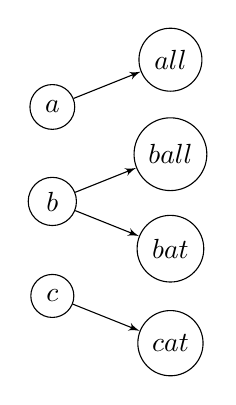
\begin{tikzpicture}
\tikzset{vertex/.style = {shape=circle,draw,minimum size=1.5em}}
\tikzset{edge/.style = {->,> = latex'}}

\node[vertex](c1) at (0,0.6) {$c$};
\node[vertex](b1) at (0,1.8) {$b$};
\node[vertex](a1) at (0,3) {$a$};
\node[vertex](d2) at (1.5,0) {$cat$};
\node[vertex](c2) at (1.5,1.2) {$bat$};
\node[vertex](b2) at (1.5,2.4) {$ball$};
\node[vertex](a2) at (1.5,3.6) {$all$};

\draw[edge] (a1) to (a2);
\draw[edge] (b1) to (b2);
\draw[edge] (b1) to (c2);
\draw[edge] (c1) to (d2);
\end{tikzpicture}
}
\pause
\subcaptionbox*{$R_{pre}$}[.5\linewidth]{
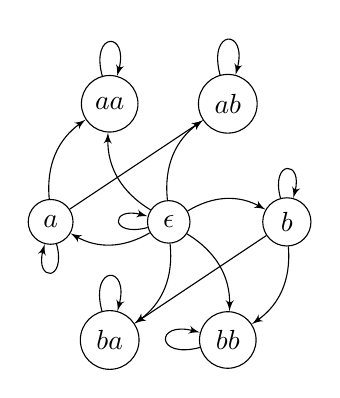
\begin{tikzpicture}
\tikzset{vertex/.style = {shape=circle,draw,minimum size=1.5em}}
\tikzset{edge/.style = {->,> = latex'}}

\node[vertex](aa) at (0.75,3) {$aa$};
\node[vertex](ab) at (2.25,3) {$ab$};
\node[vertex](a) at (0,1.5) {$a$};
\node[vertex](e) at (1.5,1.5) {$\epsilon$};
\node[vertex](b) at (3,1.5) {$b$};
\node[vertex](ba) at (0.75,0) {$ba$};
\node[vertex](bb) at (2.25,0) {$bb$};

\draw[edge] (a) to[loop below] (a);
\draw[edge] (b) to[loop above] (b);
\draw[edge] (e) to[loop left] (e);
\draw[edge] (aa) to[loop above] (aa);
\draw[edge] (ab) to[loop above] (ab);
\draw[edge] (ba) to[loop above] (ba);
\draw[edge] (bb) to[loop left] (bb);
\draw[edge] (e) to[bend left] (a);
\draw[edge] (e) to[bend left] (b);
\draw[edge] (e) to[bend left] (aa);
\draw[edge] (e) to[bend left] (ab);
\draw[edge] (e) to[bend left] (ba);
\draw[edge] (e) to[bend left] (bb);
\draw[edge] (a) to[bend left] (aa);
\draw[edge] (a) to (ab);
\draw[edge] (b) to (ba);
\draw[edge] (b) to[bend left] (bb);
\end{tikzpicture}
}
\end{figure}

\end{ex}
\end{slide}


\begin{slide}[bm=,toc=]{Reflexive Relations}
\begin{defn}{A.21}[Ben Ari]
Let $R$ be a binary relation on $S$.
\\~\\
$R$ is \emph{reflexive} if and only if $R(x,x)$ for all $x \in S$.
\end{defn}
~
\vspace{-12mm}
\pause 
\begin{figure}[t]
\caption*{\textbf{Example:} $R_{pre}$ is a reflexive relation on $S = \{\epsilon,a,b,aa,bb\}$} 
\pause 
\subcaptionbox*{As Matrix}{
$ \begin{blockarray}{cccccc}
 \begin{block}{cccccc}
  & \epsilon & a & b & aa & bb \\
 \end{block}
 \begin{block}{c[ccccc]}
 \epsilon & 1 & 1 & 1 & 1 & 1 \bigstrut[t] \\
 a        & 0 & 1 & 0 & 1 & 0  \\
 b        & 0 & 0 & 1 & 0 & 1  \\
 aa       & 0 & 0 & 0 & 1 & 0  \\
 bb       & 0 & 0 & 0 & 0 & 1  \\
 \end{block}
 \end{blockarray} $
}
\qquad
\subcaptionbox*{As Digraph}{
\pause 
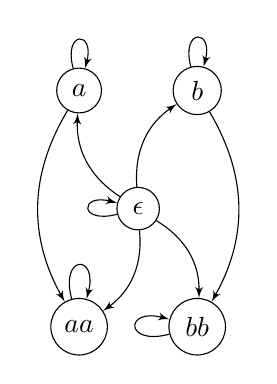
\begin{tikzpicture}
\tikzset{vertex/.style = {shape=circle,draw,minimum size=1.5em}}
\tikzset{edge/.style = {->,> = latex'}}

\node[vertex](a) at (0.75,3) {$a$};
\node[vertex](b) at (2.25,3) {$b$};
\node[vertex](e) at (1.5,1.5) {$\epsilon$};
\node[vertex](aa) at (0.75,0) {$aa$};
\node[vertex](bb) at (2.25,0) {$bb$};

\draw[edge] (a) to[loop above] (a);
\draw[edge] (b) to[loop above] (b);
\draw[edge] (e) to[loop left] (e);
\draw[edge] (aa) to[loop above] (aa);
\draw[edge] (bb) to[loop left] (bb);
\draw[edge] (e) to[bend left] (a);
\draw[edge] (e) to[bend left] (b);
\draw[edge] (e) to[bend left] (aa);
\draw[edge] (e) to[bend left] (bb);
\draw[edge] (a) to[bend right] (aa);
\draw[edge] (b) to[bend left] (bb);
\end{tikzpicture}
}
\end{figure}

\end{slide}

\begin{slide}[bm=,toc=]{Symmetric Relations}
\begin{defn}{A.21}[Ben Ari]
Let $R$ be a binary relation on $S$.
\\~\\
$R$ is \emph{symmetric} if and only if $R(x_1,x_2)$ implies $R(x_2,x_1)$.
\end{defn}
~
\vspace{-12mm}
\pause \begin{figure}[t]
\caption*{\textbf{Example:} $R_l$ is a symmetric relation on $S = \{\epsilon,a,b,aa,bb\}$} 
\pause \subcaptionbox*{As Matrix}{
$ \begin{blockarray}{cccccc}
 \begin{block}{cccccc}
  & \epsilon & a & b & aa & bb \\
 \end{block}
 \begin{block}{c[ccccc]}
 \epsilon & 1 & 0 & 0 & 0 & 0 \bigstrut[t] \\
 a        & 0 & 1 & 1 & 0 & 0  \\
 b        & 0 & 1 & 1 & 0 & 0  \\
 aa       & 0 & 0 & 0 & 1 & 1  \\
 bb       & 0 & 0 & 0 & 1 & 1  \\
 \end{block}
 \end{blockarray} $
}
\qquad
\pause \subcaptionbox*{As Digraph}{
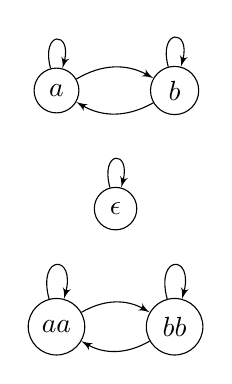
\begin{tikzpicture}
\tikzset{vertex/.style = {shape=circle,draw,minimum size=1.5em}}
\tikzset{edge/.style = {->,> = latex'}}

\node[vertex](a) at (0.75,3) {$a$};
\node[vertex](b) at (2.25,3) {$b$};
\node[vertex](e) at (1.5,1.5) {$\epsilon$};
\node[vertex](aa) at (0.75,0) {$aa$};
\node[vertex](bb) at (2.25,0) {$bb$};

\draw[edge] (a) to[loop above] (a);
\draw[edge] (b) to[loop above] (b);
\draw[edge] (e) to[loop above] (e);
\draw[edge] (aa) to[loop above] (aa);
\draw[edge] (bb) to[loop above] (bb);
\draw[edge] (a) to[bend left] (b);
\draw[edge] (b) to[bend left] (a);
\draw[edge] (bb) to[bend left] (aa);
\draw[edge] (aa) to[bend left] (bb);
\end{tikzpicture}
}
\end{figure}
\pause {\footnotesize Exercise: Give a rule for the relation.} 
\pause {\footnotesize \textbf{Ans:} $R_{l} = \{(x,y)| |x| = |y|\}$}
\end{slide}

\begin{slide}[bm=,toc=]{Antisymmetric Relations}
\begin{defn}{A.21}[Ben Ari]
Let $R$ be a binary relation on $S$.
\\~\\
$R$ is \emph{antisymmetric} if and only if $(x_1,x_2) \in R$ and $(x_2,x_1) \in
R$ implies $x_1 = x_2$.
\end{defn}
~
\vspace{-12mm}
\pause \begin{figure}[t]
\caption*{\textbf{Example:} $R_{pre}$ is also antisymmetric on $S = \{\epsilon,a,b,aa,bb\}$} 
\subcaptionbox*{As Matrix}{
\pause
$ \begin{blockarray}{cccccc}
 \begin{block}{cccccc}
  & \epsilon & a & b & aa & bb \\
 \end{block}
 \begin{block}{c[ccccc]}
 \epsilon & 1 & 1 & 1 & 1 & 1 \bigstrut[t] \\
 a        & 0 & 1 & 0 & 1 & 0  \\
 b        & 0 & 0 & 1 & 0 & 1  \\
 aa       & 0 & 0 & 0 & 1 & 0  \\
 bb       & 0 & 0 & 0 & 0 & 1  \\
 \end{block}
 \end{blockarray} $
}
\qquad
\subcaptionbox*{As Digraph}{
\pause
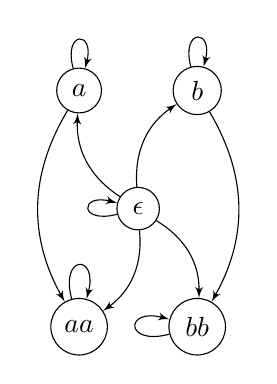
\begin{tikzpicture}
\tikzset{vertex/.style = {shape=circle,draw,minimum size=1.5em}}
\tikzset{edge/.style = {->,> = latex'}}

\node[vertex](a) at (0.75,3) {$a$};
\node[vertex](b) at (2.25,3) {$b$};
\node[vertex](e) at (1.5,1.5) {$\epsilon$};
\node[vertex](aa) at (0.75,0) {$aa$};
\node[vertex](bb) at (2.25,0) {$bb$};

\draw[edge] (a) to[loop above] (a);
\draw[edge] (b) to[loop above] (b);
\draw[edge] (e) to[loop left] (e);
\draw[edge] (aa) to[loop above] (aa);
\draw[edge] (bb) to[loop left] (bb);
\draw[edge] (e) to[bend left] (a);
\draw[edge] (e) to[bend left] (b);
\draw[edge] (e) to[bend left] (aa);
\draw[edge] (e) to[bend left] (bb);
\draw[edge] (a) to[bend right] (aa);
\draw[edge] (b) to[bend left] (bb);
\end{tikzpicture}
}
\end{figure}
\end{slide}

\begin{slide}[bm=,toc=]{Transitive Relations}
\begin{defn}{A.21}[Ben Ari]
Let $R$ be a binary relation on $S$.
\\~\\
$R$ is \emph{transitive} if and only if $R(x_1,x_2)$ and $R(x_2,x_3)$ implies $R(x_1,x_3)$.
\end{defn}
~
\vspace{-12mm}
\pause \begin{figure}[t]
\caption*{\textbf{Example:} Both $R_{pre}$ and $R_l$ are transitive on $S = \{\epsilon,a,b,aa,bb\}$} 
\subcaptionbox*{$R_{pre}$}{
\pause
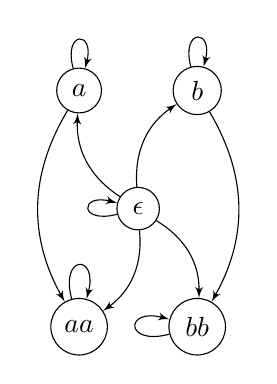
\begin{tikzpicture}
\tikzset{vertex/.style = {shape=circle,draw,minimum size=1.5em}}
\tikzset{edge/.style = {->,> = latex'}}

\node[vertex](a) at (0.75,3) {$a$};
\node[vertex](b) at (2.25,3) {$b$};
\node[vertex](e) at (1.5,1.5) {$\epsilon$};
\node[vertex](aa) at (0.75,0) {$aa$};
\node[vertex](bb) at (2.25,0) {$bb$};

\draw[edge] (a) to[loop above] (a);
\draw[edge] (b) to[loop above] (b);
\draw[edge] (e) to[loop left] (e);
\draw[edge] (aa) to[loop above] (aa);
\draw[edge] (bb) to[loop left] (bb);
\draw[edge] (e) to[bend left] (a);
\draw[edge] (e) to[bend left] (b);
\draw[edge] (e) to[bend left] (aa);
\draw[edge] (e) to[bend left] (bb);
\draw[edge] (a) to[bend right] (aa);
\draw[edge] (b) to[bend left] (bb);
\end{tikzpicture}
}
\qquad
\subcaptionbox*{$R_l$}{
\pause
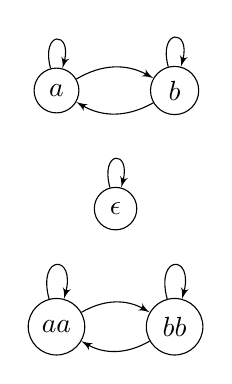
\begin{tikzpicture}
\tikzset{vertex/.style = {shape=circle,draw,minimum size=1.5em}}
\tikzset{edge/.style = {->,> = latex'}}

\node[vertex](a) at (0.75,3) {$a$};
\node[vertex](b) at (2.25,3) {$b$};
\node[vertex](e) at (1.5,1.5) {$\epsilon$};
\node[vertex](aa) at (0.75,0) {$aa$};
\node[vertex](bb) at (2.25,0) {$bb$};

\draw[edge] (a) to[loop above] (a);
\draw[edge] (b) to[loop above] (b);
\draw[edge] (e) to[loop above] (e);
\draw[edge] (aa) to[loop above] (aa);
\draw[edge] (bb) to[loop above] (bb);
\draw[edge] (a) to[bend left] (b);
\draw[edge] (b) to[bend left] (a);
\draw[edge] (bb) to[bend left] (aa);
\draw[edge] (aa) to[bend left] (bb);
\end{tikzpicture}
}
\end{figure}
\end{slide}
\begin{slide}[bm=,toc=]{Equivalence Relations}
\begin{defn}{--- Equivalence Relations}~\\
A relation is an equivalence relation if it is:

\begin{itemize}
\item<2-> Reflexive
\item<3-> Symmetric
\item<4-> Transitive
\end{itemize}
\end{defn}
\pause[4]
\textbf{Examples}:
\begin{itemize}
\item<6-> $\{(x,y) | x = y \}$
\item<7-> $\{(x,y) | x \text{ and } y \text{ begin with the same character}\}$
\item<8-> $\{(x,y) | x \text{ and } y \text{ contain the same substring}\}$
\item<9-> $R_{l}$ 
\end{itemize}
\end{slide}

\begin{slide}[bm=,toc=]{Equivalence Classes}
\begin{defn}{--- Equivalence Classes}~\\
Let $E$ be an equivalence relation on a set $S$. 
~\\
\pause
For any element $x \in S$:
\begin{itemize}
\item<3-> We define the \emph{equivalence class} of $x$ as the set of elements in
      $S$ that are related to $x$ under relation $E$.
\item<4-> The equivalence class of $x$ is denoted $[x]_{E}$ (or simply $[x]$ if
      the relation is clear from context).
\item<5-> In symbols, $[x] = \{y \in S| (x,y) \in E\}$
\end{itemize}
\end{defn}
~\\
\pause[4]
\begin{thm}{ -- $S$ is the union of its equivalence classes}~\\
\pause
Let $E$ be an equivalence relation on a set $S$. Then
\pause
\[
  \bigcup_{x \in X} [x]_E = S
  \]
\end{thm}
\pause
This follows from the fact that $E$ is reflexive.
\end{slide}

\begin{slide}[bm=,toc=]{Equivalence Classes Partition a Set}
\begin{thm}{ -- Equivalence classes are equal or disjoint}~\\
\pause
The following are equivalent:
\begin{itemize}
\item<3-> $xEy$ 
\item<4-> $[x] = [y]$ 
\item<5-> $[x] \cap [y] \neq \emptyset$ 
\end{itemize}
\pause[4]
Consquently, if $x$ and $y$ are not related by $E$, then:
\item<7->$[x] \neq [y]$, and
\item<8->$[x] \cap [y] = \emptyset$.
\end{thm}
\pause[3]
Colloquially, equivalence classes cannot partially overlap. 
\pause
\vspace{5mm}
\begin{thm}{ -- Equivalence classes partition a set}~\\
\pause
This follows directly from two preceding theorems. 
\end{thm}
\end{slide}

\begin{slide}[bm=,toc=]{Partial Orders}
\begin{defn}{--- Partial Orders}~\\
\pause
A relation is a partial order if it is:

\begin{itemize}
\item<3-> Reflexive
\item<4-> Antisymmetric
\item<5-> Transitive
\end{itemize}
\end{defn}
\pause[4]
\textbf{Examples}:
\begin{itemize}
\item<7-> $R_{pre}$
\item<8-> $\{(x,y) | x \text{ is a substring of } y \}$
\item<9-> $\{(x,y) | x \text{ is a subset of } y \}$
\item<10-> $\{(x,y) | y \text{ is a suffix of } x \}$
\end{itemize}
\end{slide}
\begin{slide}[bm=,toc=]{Combining Relations}
Recall that relations are sets.
\\~\\
\pause
\textbf{Consequently:}~\\
\begin{itemize}
\item<3-> Relations can be combined using set operations.
\item<4-> That is, given arbitrary relations $R_1$ and $R_2$, we can form:
\begin{itemize}
\item<5-> $R_1 \cup R_2$
\item<6-> $R_1 \cap R_2$
\item<7-> $R_1 - R_2$
\item<8-> $R_2 - R_1$
\end{itemize}
\item<9-> Note that we generally expect $R_1$ and $R_2$ to have the same arity.
\end{itemize}
\end{slide}

\begin{slide}[bm=,toc=]{Composition of Binary Relations}
We can also combine binary relations using the \emph{composition} operation, denoted
$R_1 \circ R_2$.
\begin{itemize}
\item<2-> Assume $R_2$ is a relation on $S_1 \times S_2$ and $R_1$ is a relation on
$S_3 \times S_4$.
\item<3-> Let $S = S_2 \cap S_3$.
\item<4-> The composition forms a new relation on $S_1 \times S_4$, such that:
\begin{itemize}
\item<5-> $(x,z) \in R_1 \circ R_2$ if and only if there exists $y$ in $S$ such
that $(y,z) \in R_1$ and $(x,y) \in R_2$.
\end{itemize}
\item<6-> Note that in the case where $S = \emptyset$, $R_1 \circ R_2$ is also empty.
\end{itemize}

\vspace{-5mm}
\begin{figure}[b]
\begin{subfigure}{.4\linewidth}
\pause[6]
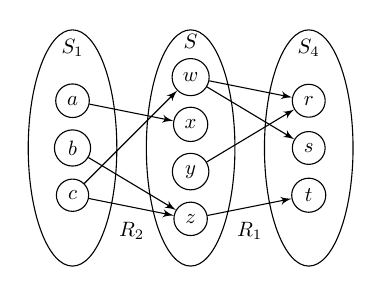
\begin{tikzpicture}[scale=.75, every node/.style={scale=.75}]
\tikzset{vertex/.style = {shape=circle,draw,minimum size=1.5em}}
\tikzset{edge/.style = {->,> = latex'}}

\draw (0, 1.2) ellipse (.75cm and 2cm);
\node[vertex](c) at (0,0.4) {$c$};
\node[vertex](b) at (0,1.2) {$b$};
\node[vertex](a) at (0,2) {$a$};
\node (s1) at (0, 2.9) {$S_1$};

\node (r2) at (1, -0.2) {$R_2$};

\draw (2, 1.2) ellipse (.75cm and 2cm);
\node[vertex](z) at (2,0) {$z$};
\node[vertex](y) at (2,0.8) {$y$};
\node[vertex](x) at (2,1.6) {$x$};
\node[vertex](w) at (2,2.4) {$w$};
\node (s) at (2, 3) {$S$};

\node (r1) at (3, -0.2) {$R_1$};

\draw (4, 1.2) ellipse (.75cm and 2cm);
\node[vertex](t) at (4,0.4) {$t$};
\node[vertex](s) at (4,1.2) {$s$};
\node[vertex](r) at (4,2) {$r$};
\node (s4) at (4, 2.9) {$S_4$};



\draw[edge] (a) to (x);
\draw[edge] (b) to (z);
\draw[edge] (c) to (w);
\draw[edge] (c) to (z);

\draw[edge] (w) to (r);
\draw[edge] (w) to (s);
\draw[edge] (z) to (t);
\draw[edge] (y) to (r);

\end{tikzpicture}

\end{subfigure}
\begin{subfigure}{.5\linewidth}
\pause
\begin{align*}
  =& R_1 \circ R_2 \\
  =& \{(b,t),(c,r),(c,s),(c,t)\}
\end{align*}
\end{subfigure}
\end{figure}

\end{slide}
\begin{slide}[bm=,toc=]{Powers of Binary Relations}
\begin{defn}{-- Powers of Relations}
~\\
\pause
Let $R$ be a binary homogenous relation on $S$.
\\~\\
\pause
The relation $R^n$ is defined inductively by: 
\begin{itemize}
\item<4-> $R^1 = R$
\item<5-> $R^{n+1} = R^n \circ R$
\end{itemize}
\end{defn}
\pause[3]
\textbf{Notes:}
\begin{itemize}
\item<7-> This definition makes use of the concept of relation composition
given on the previous slide.
\item<8->Useful for defining paths of length $n$.
\item<9->We will see it again in modal logic.
\end{itemize}
\end{slide}



\section[slide=true]{Functions}
\begin{slide}[bm=,toc=]{Definition}
\begin{defn}{A.23}[Ben Ari]
~\\
Let $\mathcal{F}$ be a relation on $S_1 \times \cdots \times S_n$.
\\~\\
\pause
$\mathcal{F}$ is a \emph{function} if and only if for every \emph{(n -- 1)-tuple}
$(x_1,...,x_{n-1}) \in S_1 \times \cdots \times S_{n-1}$, there is at most
one $x_n \in S_n$, such that $\mathcal{F}(x_1,...,x_n)$.
\begin{itemize}
\item<3-> For a function $\mathcal{F}$ we write $x_n = \mathcal{F}(x_1,...,x_{n-1})$.
\item<4-> The \emph{domain} of $\mathcal{F}$ is the set of all
$(x_1,...,x_{n-1})\in S_1 \times \cdots \times S_{n-1}$ for which (exactly one)
$x_n = \mathcal{F}(x_1,...,x_{n-1})$ exists.
\item<5->The \emph{range} of $\mathcal{F}$ is the set of all $x_n \in S_n$ such
that $x_n = \mathcal{F}(x_1,...,x_{n-1})$ for at least one $(x_1,...,x_{n-1})$. 
\end{itemize}
\end{defn}
\end{slide}

\begin{slide}[bm=,toc=]{Examples of Functions}
\textbf{As a Special Relation:}
\begin{itemize}
\item<2-> With explicit set notation: \[f_1 = \{(1,3),(2,1),(3,2)\}\]
\vspace{-5mm}
\item<3-> With set comprehension: \[f_2 = \{(n_1,n_2)|n_2 = n_1^2\}\]
\end{itemize}
\pause[3]
\textbf{Functional Notation:}
\vspace{-3mm}
\[
  f_3(x) = x^2 + 1
  \]
\vspace{-5mm}
\pause
\textbf{Arrow Notation:}
\vspace{-3mm}
\begin{align*}
f_4:\N &\longrightarrow \R \\
    x &\mapsto \sqrt{x}
\end{align*}

\end{slide}

\begin{slide}[bm=,toc=]{Total and Partial Functions}
\begin{defn}{A.23}[Ben Ari]~\\
\pause
\vspace{2mm}
$\mathcal{F}$ is \emph{total} if the domain of $\mathcal{F}$ is (all of)
  $S_1 \times \cdots \times S_{n-1}$;\\
\pause
\vspace{2mm}
Otherwise, $\mathcal{F}$ is \emph{partial}.
\end{defn}

\begin{figure}[b]
\subcaptionbox*{Total Function}[.4\linewidth]{
\pause
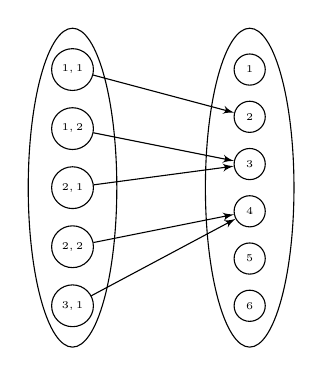
\begin{tikzpicture}[scale=.75, every node/.style={scale=.75}]
\tikzset{vertex/.style = {shape=circle,draw,minimum size=1.5em}}
\tikzset{edge/.style = {->,> = latex'}}

\draw (0, 2) ellipse (0.75cm and 2.7cm);

\node[vertex](a5) at (0,0) {\tiny $3,1$};
\node[vertex](a4) at (0,1) {\tiny $2,2$};
\node[vertex](a3) at (0,2) {\tiny $2,1$};
\node[vertex](a2) at (0,3) {\tiny $1,2$};
\node[vertex](a1) at (0,4) {\tiny $1,1$};

\draw (3, 2) ellipse (0.75cm and 2.7cm);

\node[vertex](b6) at (3,0)   {\tiny  $6$};
\node[vertex](b5) at (3,0.8) {\tiny  $5$};
\node[vertex](b4) at (3,1.6) {\tiny  $4$};
\node[vertex](b3) at (3,2.4) {\tiny  $3$};
\node[vertex](b2) at (3,3.2) {\tiny  $2$};
\node[vertex](b1) at (3,4) {\tiny    $1$};

\draw[edge] (a1) to (b2);
\draw[edge] (a2) to (b3);
\draw[edge] (a3) to (b3);
\draw[edge] (a4) to (b4);
\draw[edge] (a5) to (b4);

\end{tikzpicture}
}
\qquad
\subcaptionbox*{Partial Function}[.4\linewidth]{
\pause
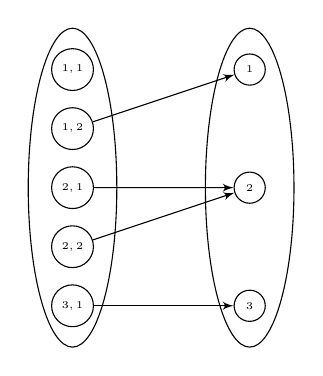
\begin{tikzpicture}[scale=.75, every node/.style={scale=.75}]
\tikzset{vertex/.style = {shape=circle,draw,minimum size=1.5em}}
\tikzset{edge/.style = {->,> = latex'}}
\draw (0, 2) ellipse (0.75cm and 2.7cm);

\node[vertex](a5) at (0,0) {\tiny $3,1$};
\node[vertex](a4) at (0,1) {\tiny $2,2$};
\node[vertex](a3) at (0,2) {\tiny $2,1$};
\node[vertex](a2) at (0,3) {\tiny $1,2$};
\node[vertex](a1) at (0,4) {\tiny $1,1$};

\draw (3, 2) ellipse (0.75cm and 2.7cm);

\node[vertex](b3) at (3,0)   {\tiny  $3$};
\node[vertex](b2) at (3,2) {\tiny  $2$};
\node[vertex](b1) at (3,4) {\tiny  $1$};

\draw[edge] (a2) to (b1);
\draw[edge] (a3) to (b2);
\draw[edge] (a4) to (b2);
\draw[edge] (a5) to (b3);

\end{tikzpicture}
}

\end{figure}

\end{slide}

\begin{slide}[bm=,toc=]{Injective / one-to-one Functions}
\begin{defn}{A.23}[Ben Ari]~\\
\vspace{2mm}
$\mathcal{F}$ is \emph{injective} or \emph{one-to-one} if and only if:
\begin{itemize}
\item<2-> $(x_1,...,x_{n-1}) \neq (y_1,...,y_{n-1})$
\end{itemize}
\pause[2]
implies
\begin{itemize}
\item<4-> $\mathcal{F}(x_1,...,x_{n-1}) \neq \mathcal{F}(y_1,...,y_{n-1})$
\end{itemize}
\end{defn}

\vspace{-6mm}
\begin{figure}[b]
\subcaptionbox*{Injective}[.4\linewidth]{
\pause[2]
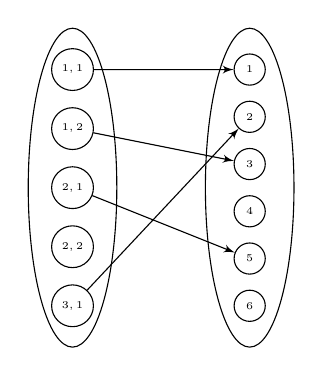
\begin{tikzpicture}[scale=.75, every node/.style={scale=.75}]
\tikzset{vertex/.style = {shape=circle,draw,minimum size=1.5em}}
\tikzset{edge/.style = {->,> = latex'}}

\draw (0, 2) ellipse (0.75cm and 2.7cm);

\node[vertex](a5) at (0,0) {\tiny $3,1$};
\node[vertex](a4) at (0,1) {\tiny $2,2$};
\node[vertex](a3) at (0,2) {\tiny $2,1$};
\node[vertex](a2) at (0,3) {\tiny $1,2$};
\node[vertex](a1) at (0,4) {\tiny $1,1$};

\draw (3, 2) ellipse (0.75cm and 2.7cm);

\node[vertex](b6) at (3,0)   {\tiny  $6$};
\node[vertex](b5) at (3,0.8) {\tiny  $5$};
\node[vertex](b4) at (3,1.6) {\tiny  $4$};
\node[vertex](b3) at (3,2.4) {\tiny  $3$};
\node[vertex](b2) at (3,3.2) {\tiny  $2$};
\node[vertex](b1) at (3,4) {\tiny    $1$};

\draw[edge] (a1) to (b1);
\draw[edge] (a2) to (b3);
\draw[edge] (a3) to (b5);
\draw[edge] (a5) to (b2);
\end{tikzpicture}
}
\qquad
\subcaptionbox*{Not Injective}[.4\linewidth]{
\pause
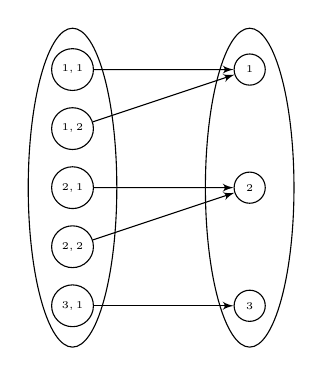
\begin{tikzpicture}[scale=.75, every node/.style={scale=.75}]
\tikzset{vertex/.style = {shape=circle,draw,minimum size=1.5em}}
\tikzset{edge/.style = {->,> = latex'}}
\draw (0, 2) ellipse (0.75cm and 2.7cm);

\node[vertex](a5) at (0,0) {\tiny $3,1$};
\node[vertex](a4) at (0,1) {\tiny $2,2$};
\node[vertex](a3) at (0,2) {\tiny $2,1$};
\node[vertex](a2) at (0,3) {\tiny $1,2$};
\node[vertex](a1) at (0,4) {\tiny $1,1$};

\draw (3, 2) ellipse (0.75cm and 2.7cm);

\node[vertex](b3) at (3,0)   {\tiny  $3$};
\node[vertex](b2) at (3,2) {\tiny  $2$};
\node[vertex](b1) at (3,4) {\tiny  $1$};

\draw[edge] (a1) to (b1);
\draw[edge] (a2) to (b1);
\draw[edge] (a3) to (b2);
\draw[edge] (a4) to (b2);
\draw[edge] (a5) to (b3);

\end{tikzpicture}
}

\end{figure}


\end{slide}

\begin{slide}[bm=,toc=]{Surjective / onto Functions}
\begin{defn}{A.23}[Ben Ari]~\\
\vspace{2mm}
$\mathcal{F}$ is \emph{surjective} or \emph{onto} if and only if its range is all of $S_n$.\\
\vspace{2mm}
\pause
Equivalently, $\mathcal{F}$ from $S_1$ to $S_2$ is \emph{surjective} if 
and only if for all $y \in S_2$ there is an $x \in S_1$ such that
$\mathcal{F}(x) = y$. 
\end{defn}
\vspace{-5mm}
\begin{figure}[b]
\subcaptionbox*{Surjective}[.4\linewidth]{
\pause
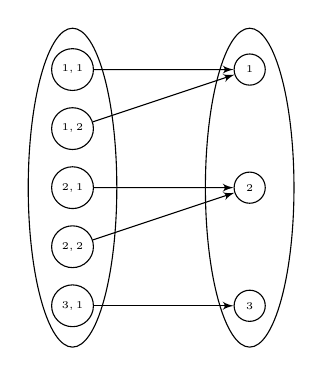
\begin{tikzpicture}[scale=.75, every node/.style={scale=.75}]
\tikzset{vertex/.style = {shape=circle,draw,minimum size=1.5em}}
\tikzset{edge/.style = {->,> = latex'}}
\draw (0, 2) ellipse (0.75cm and 2.7cm);

\node[vertex](a5) at (0,0) {\tiny $3,1$};
\node[vertex](a4) at (0,1) {\tiny $2,2$};
\node[vertex](a3) at (0,2) {\tiny $2,1$};
\node[vertex](a2) at (0,3) {\tiny $1,2$};
\node[vertex](a1) at (0,4) {\tiny $1,1$};

\draw (3, 2) ellipse (0.75cm and 2.7cm);

\node[vertex](b3) at (3,0)   {\tiny  $3$};
\node[vertex](b2) at (3,2) {\tiny  $2$};
\node[vertex](b1) at (3,4) {\tiny  $1$};

\draw[edge] (a1) to (b1);
\draw[edge] (a2) to (b1);
\draw[edge] (a3) to (b2);
\draw[edge] (a4) to (b2);
\draw[edge] (a5) to (b3);

\end{tikzpicture}
}
\qquad
\subcaptionbox*{Not Surjective}[.4\linewidth]{
\pause
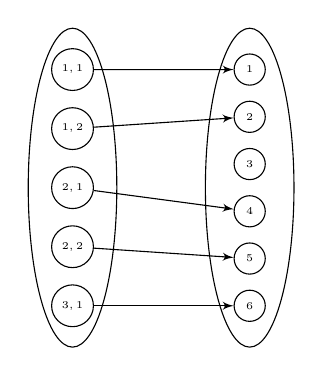
\begin{tikzpicture}[scale=.75, every node/.style={scale=.75}]
\tikzset{vertex/.style = {shape=circle,draw,minimum size=1.5em}}
\tikzset{edge/.style = {->,> = latex'}}

\draw (0, 2) ellipse (0.75cm and 2.7cm);

\node[vertex](a5) at (0,0) {\tiny $3,1$};
\node[vertex](a4) at (0,1) {\tiny $2,2$};
\node[vertex](a3) at (0,2) {\tiny $2,1$};
\node[vertex](a2) at (0,3) {\tiny $1,2$};
\node[vertex](a1) at (0,4) {\tiny $1,1$};

\draw (3, 2) ellipse (0.75cm and 2.7cm);

\node[vertex](b6) at (3,0)   {\tiny  $6$};
\node[vertex](b5) at (3,0.8) {\tiny  $5$};
\node[vertex](b4) at (3,1.6) {\tiny  $4$};
\node[vertex](b3) at (3,2.4) {\tiny  $3$};
\node[vertex](b2) at (3,3.2) {\tiny  $2$};
\node[vertex](b1) at (3,4) {\tiny    $1$};

\draw[edge] (a1) to (b1);
\draw[edge] (a2) to (b2);
\draw[edge] (a3) to (b4);
\draw[edge] (a4) to (b5);
\draw[edge] (a5) to (b6);

\end{tikzpicture}
}

\end{figure}

\end{slide}

\begin{slide}[bm=,toc=]{Bijective Functions}
\begin{defn}{A.23}[Ben Ari]~\\
$\mathcal{F}$ is \emph{bijective} or \emph{one-to-one and onto} if and only if
it is injective and surjective.
\end{defn}

\begin{figure}[b]
\pause
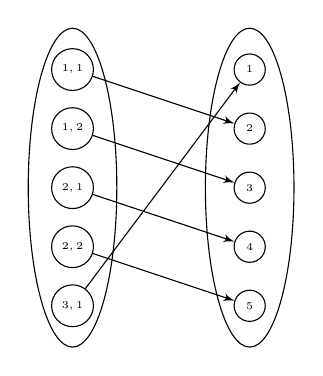
\begin{tikzpicture}[scale=.75, every node/.style={scale=.75}]
\tikzset{vertex/.style = {shape=circle,draw,minimum size=1.5em}}
\tikzset{edge/.style = {->,> = latex'}}

\draw (0, 2) ellipse (0.75cm and 2.7cm);

\node[vertex](a5) at (0,0) {\tiny $3,1$};
\node[vertex](a4) at (0,1) {\tiny $2,2$};
\node[vertex](a3) at (0,2) {\tiny $2,1$};
\node[vertex](a2) at (0,3) {\tiny $1,2$};
\node[vertex](a1) at (0,4) {\tiny $1,1$};

\draw (3, 2) ellipse (0.75cm and 2.7cm);

\node[vertex](b5) at (3,0) {\tiny  $5$};
\node[vertex](b4) at (3,1) {\tiny  $4$};
\node[vertex](b3) at (3,2) {\tiny  $3$};
\node[vertex](b2) at (3,3) {\tiny  $2$};
\node[vertex](b1) at (3,4) {\tiny  $1$};

\draw[edge] (a1) to (b2);
\draw[edge] (a2) to (b3);
\draw[edge] (a3) to (b4);
\draw[edge] (a4) to (b5);
\draw[edge] (a5) to (b1);

\end{tikzpicture}
\caption*{Bijective Function}
\end{figure}

\end{slide}

\begin{slide}[bm=,toc=]{Composition of Functions}
As with relations, we can combine functions using the \emph{composition} operation, 
denoted $f \circ g$.
\begin{itemize}
\item<2-> Assume $g$ is a function from $S_1$ to $S_2$ and $f$ is a function from 
$S_3$ to $S_4$ and let $S = S_2 \cap S_3$.
\item<3->The composition forms a new function on $S_1 \times S_4$, such that:
\[
  f \circ g(x) = f(g(x))
\]
\vspace{-5mm}
\item<4-> \textbf{Note:} since functions are relations, the above follows immediately from
the definition of composition of relations.
\end{itemize}
\vspace{-5mm}
\begin{figure}[b]
\pause[4]
\begin{subfigure}{.3\linewidth}
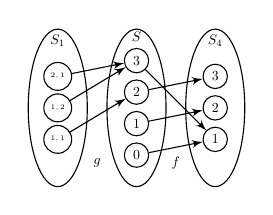
\begin{tikzpicture}[scale=.5, every node/.style={scale=.5}]
\tikzset{vertex/.style = {shape=circle,draw,minimum size=1.5em}}
\tikzset{edge/.style = {->,> = latex'}}

\draw (0, 1.2) ellipse (.75cm and 2cm);
\node[vertex](c) at (0,0.4) {\tiny $1,1$};
\node[vertex](b) at (0,1.2) {\tiny $1,2$};
\node[vertex](a) at (0,2)   {\tiny $2,1$};
\node (s1) at (0, 2.9) {$S_1$};

\node (g) at (1, -0.2) {$g$};

\draw (2, 1.2) ellipse (.75cm and 2cm);
\node[vertex](0) at (2,0) {$0$};
\node[vertex](1) at (2,0.8) {$1$};
\node[vertex](2) at (2,1.6) {$2$};
\node[vertex](3) at (2,2.4) {$3$};
\node (s) at (2, 3) {$S$};

\node (f) at (3, -0.2) {$f$};

\draw (4, 1.2) ellipse (.75cm and 2cm);
\node[vertex](b1) at (4,0.4) {$1$};
\node[vertex](b2) at (4,1.2) {$2$};
\node[vertex](b3) at (4,2)   {$3$};
\node (s4) at (4, 2.9) {$S_4$};

\draw[edge] (a) to (3);
\draw[edge] (b) to (3);
\draw[edge] (c) to (2);

\draw[edge] (0) to (b1);
\draw[edge] (1) to (b2);
\draw[edge] (2) to (b3);
\draw[edge] (3) to (b1);

\end{tikzpicture}

\end{subfigure}
\pause
\begin{subfigure}{.3\linewidth}
\begin{align*}
  f(x)       &= x \pmod{3} + 1 \\
  g(x_1,x_2) &= x_1 + x_2 \\
  f \circ g(x_1,x_2) &= f(g(x_1,x_2)) \\
                     &= (x_1 + x_2) \pmod{3} + 1
\end{align*}
\end{subfigure}
\end{figure}
\end{slide}


\end{document}

